\documentclass{article}

\usepackage[margin=2cm]{geometry}
\usepackage[latin1]{inputenc}
\usepackage{todo}
\usepackage{url}
\usepackage{caption}
\usepackage{subcaption}
\usepackage{graphicx}

\title{Fractal Drums}

\author{Knut Andre G. Prestsveen}

\begin{document}
\maketitle

\section{Abstract}
A numerical study of vibrations of quadratic Koch fractal shaped drums. For any drum, it's size is related to the pitch it makes, the larger the area, the lower the pitch. The question in mind now, is if the shape of the drum also affects the tone, and this study computes the eigenstates of a fractal drum with finite differences. The resulting resulting density of states is compared with the findings of the Weyl-Berry-conjecture and results for a drum with continous perimeter of the same
area.

\section{Theory}
\subsection{The Weyl-conjecture}
The shape of the drum cannot be completely inferred from it's sound alone, but some information can be extracted. Firstly the area of the drum $A$ can be found from

\begin{equation}
    \label{area}
    A = 4*\pi ...,
\end{equation}
where $N(\omega)$ is the integrated density of states (IDOS), i.e. the number of eigenfrequencies smaller than the frequency $\omega$. Also Hermann Weyl conjectured that the second term in the asymptotic of $N(\omega)$ gives the length of the drums perimeter $L$, so that

\begin{equation}
    \label{weyl-conjecture}
    N(\omega) = \frac{A}{4*\pi}...
\end{equation}
in the limit of large $\omega$. Equation \ref{weyl-conjecture} is the Weyl-conjecture for the IDOS, and is proven correct under the assumption of a smooth boundary. This study tries to see what happens when the boundary is fractal.

\subsection{Quadratic Koch Fractal}
Describe qkf, recursive generation etc.

\subsection{Finite Difference Approximation}
Five-point and nine-point stensil. Equations...

\section{Code}
Cool code snippets and text explaining the implementation.

\section{Results}
Cool plots, and hopefully something clever about IDOS (If I am able to compute something sensible).

\begin{figure}
    \begin{subfigure}{0.3\textwidth}
        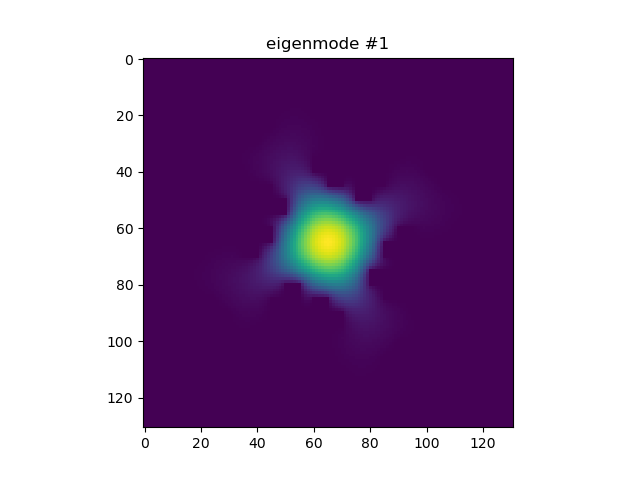
\includegraphics[width=\linewidth]{../figs/eigenmode_2d1.png}
    \end{subfigure}
    \begin{subfigure}{0.3\textwidth}
        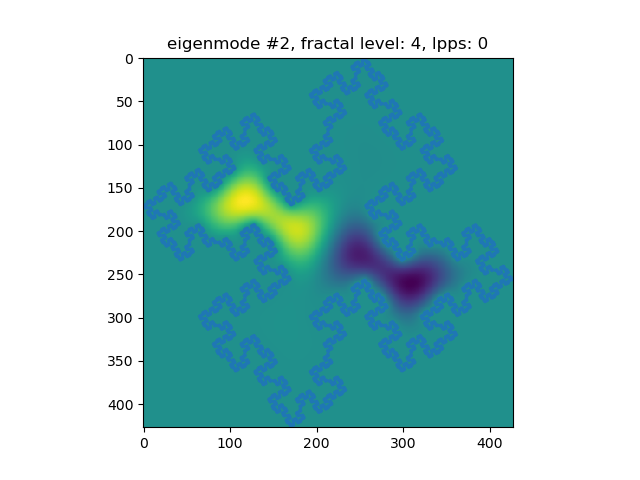
\includegraphics[width=\linewidth]{../figs/eigenmode_2d2.png}
    \end{subfigure}
    \begin{subfigure}{0.3\textwidth}
        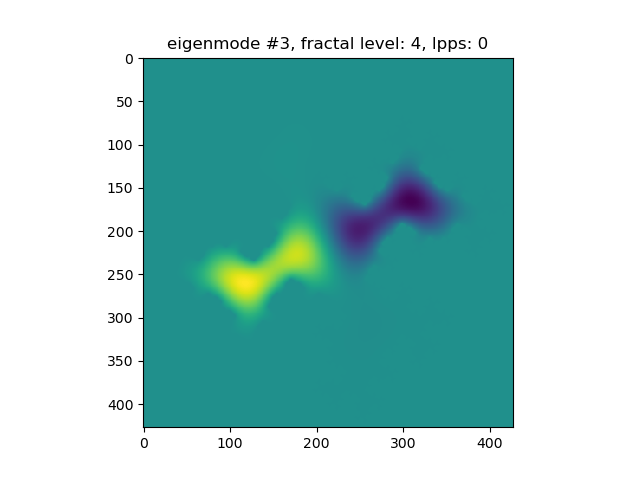
\includegraphics[width=\linewidth]{../figs/eigenmode_2d3.png}
    \end{subfigure}
    \begin{subfigure}{0.3\textwidth}
        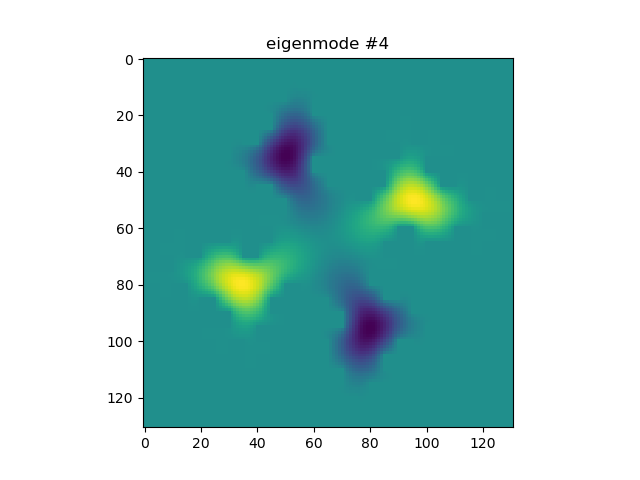
\includegraphics[width=\linewidth]{../figs/eigenmode_2d4.png}
    \end{subfigure}
    \begin{subfigure}{0.3\textwidth}
        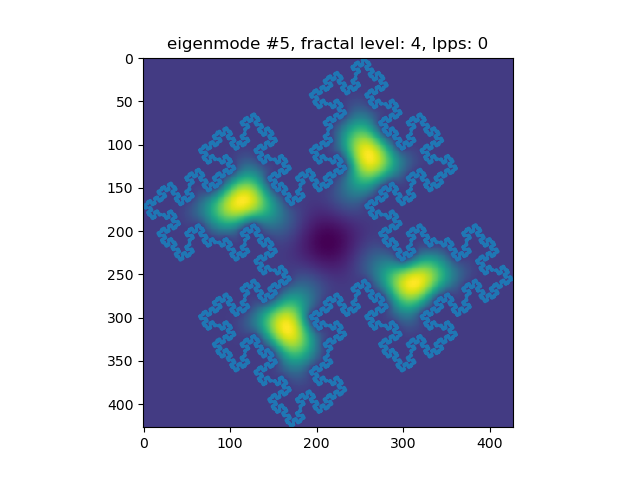
\includegraphics[width=\linewidth]{../figs/eigenmode_2d5.png}
    \end{subfigure}
    \begin{subfigure}{0.3\textwidth}
        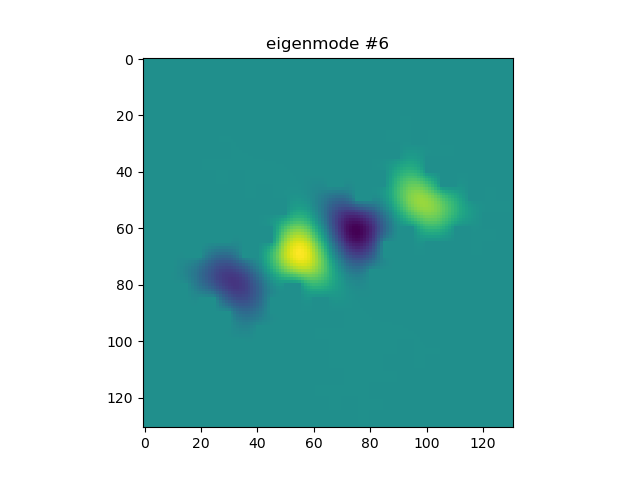
\includegraphics[width=\linewidth]{../figs/eigenmode_2d6.png}
    \end{subfigure}
    \begin{subfigure}{0.3\textwidth}
        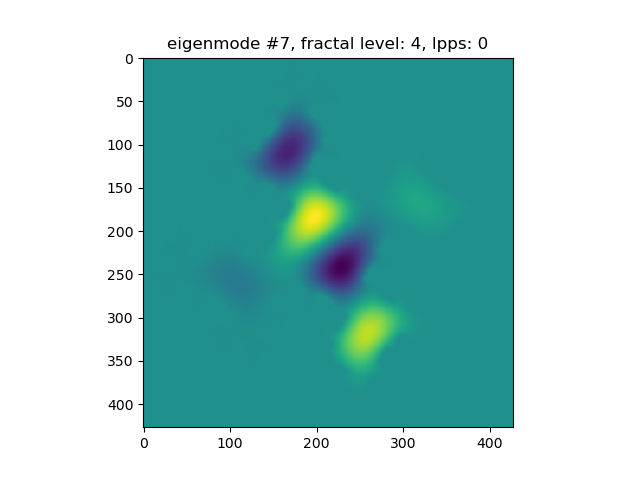
\includegraphics[width=\linewidth]{../figs/eigenmode_2d7.png}
    \end{subfigure}
    \begin{subfigure}{0.3\textwidth}
        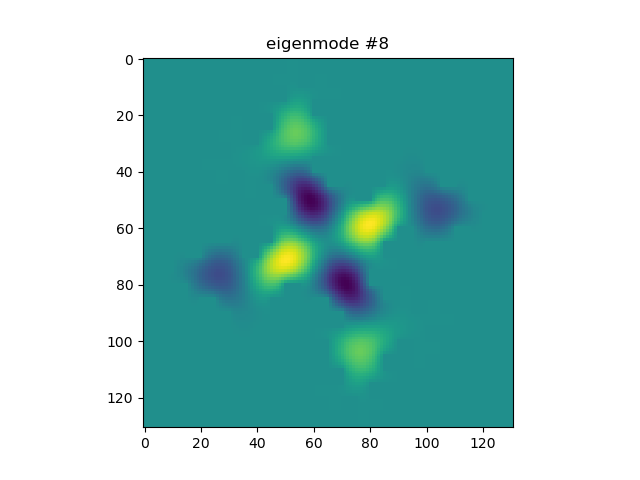
\includegraphics[width=\linewidth]{../figs/eigenmode_2d8.png}
    \end{subfigure}
    \begin{subfigure}{0.3\textwidth}
        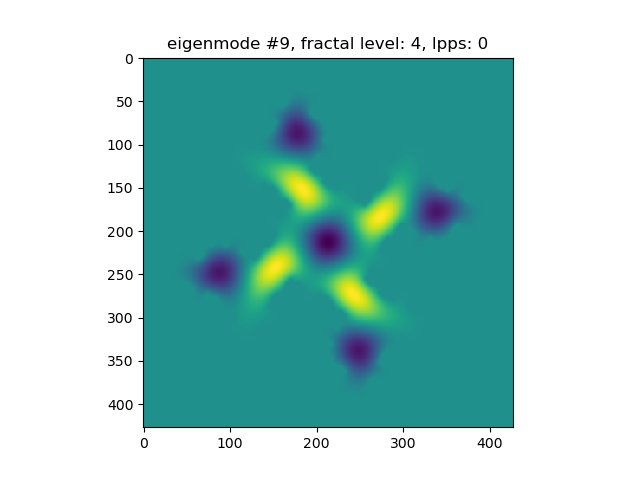
\includegraphics[width=\linewidth]{../figs/eigenmode_2d9.png}
    \end{subfigure}
    \begin{subfigure}{0.3\textwidth}
        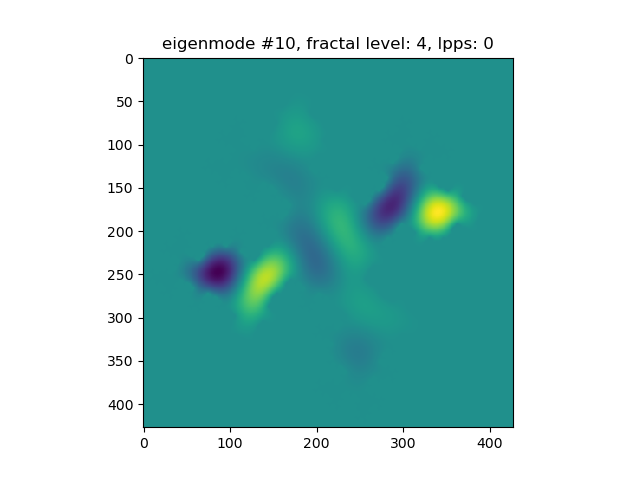
\includegraphics[width=\linewidth]{../figs/eigenmode_2d10.png}
    \end{subfigure}
    \caption{The 10 lowest eigenmodes, 2D plots.}
    \label{2dmodes}
\end{figure}

\begin{figure}
    \begin{subfigure}{0.3\textwidth}
        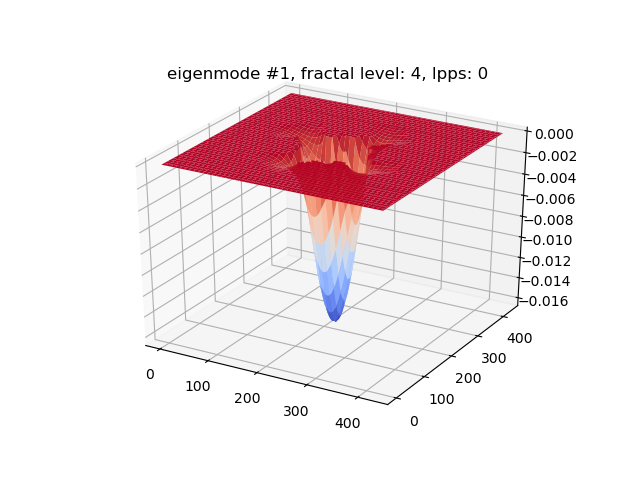
\includegraphics[width=\linewidth]{../figs/eigenmode_3d1.png}
    \end{subfigure}
    \begin{subfigure}{0.3\textwidth}
        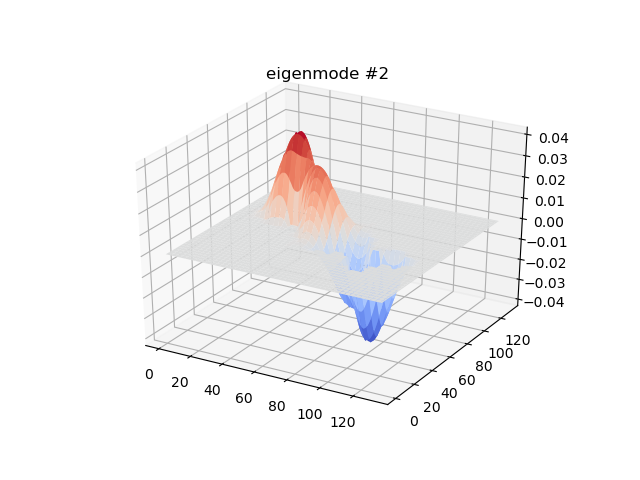
\includegraphics[width=\linewidth]{../figs/eigenmode_3d2.png}
    \end{subfigure}
    \begin{subfigure}{0.3\textwidth}
        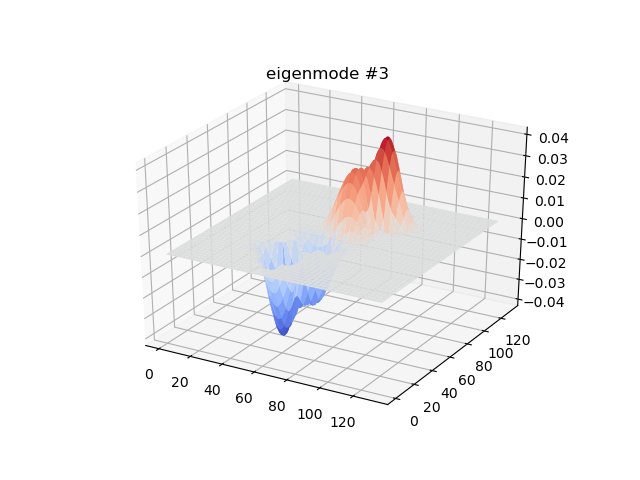
\includegraphics[width=\linewidth]{../figs/eigenmode_3d3.png}
    \end{subfigure}
    \begin{subfigure}{0.3\textwidth}
        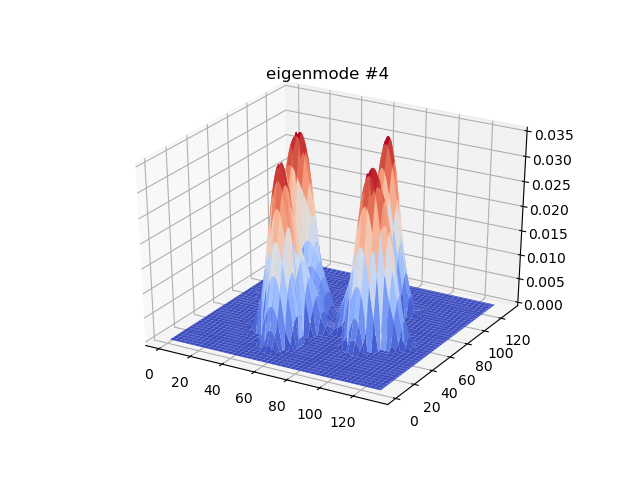
\includegraphics[width=\linewidth]{../figs/eigenmode_3d4.png}
    \end{subfigure}
    \begin{subfigure}{0.3\textwidth}
        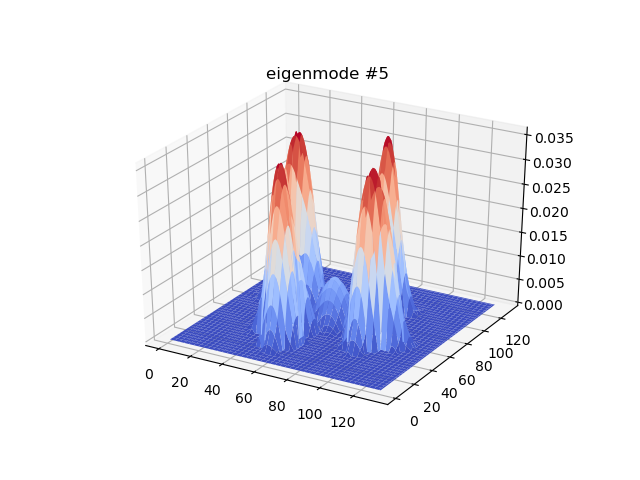
\includegraphics[width=\linewidth]{../figs/eigenmode_3d5.png}
    \end{subfigure}
    \begin{subfigure}{0.3\textwidth}
        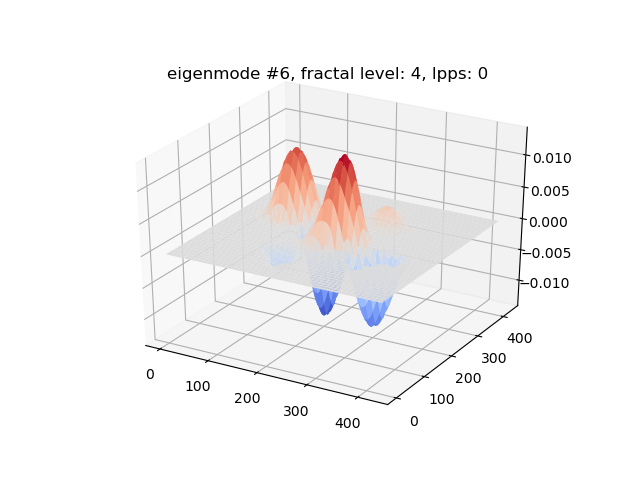
\includegraphics[width=\linewidth]{../figs/eigenmode_3d6.png}
    \end{subfigure}
    \begin{subfigure}{0.3\textwidth}
        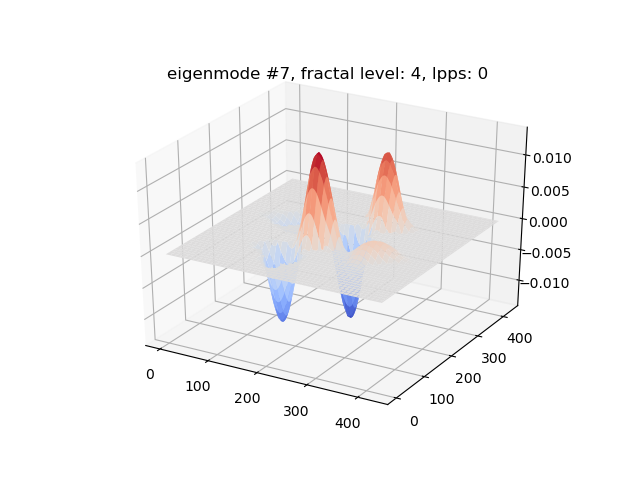
\includegraphics[width=\linewidth]{../figs/eigenmode_3d7.png}
    \end{subfigure}
    \begin{subfigure}{0.3\textwidth}
        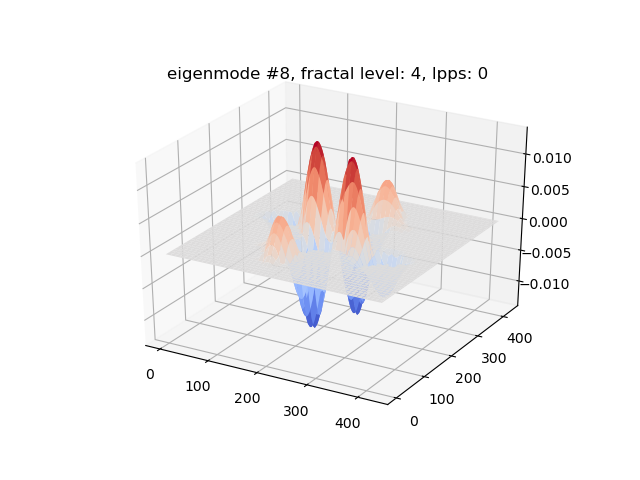
\includegraphics[width=\linewidth]{../figs/eigenmode_3d8.png}
    \end{subfigure}
    \begin{subfigure}{0.3\textwidth}
        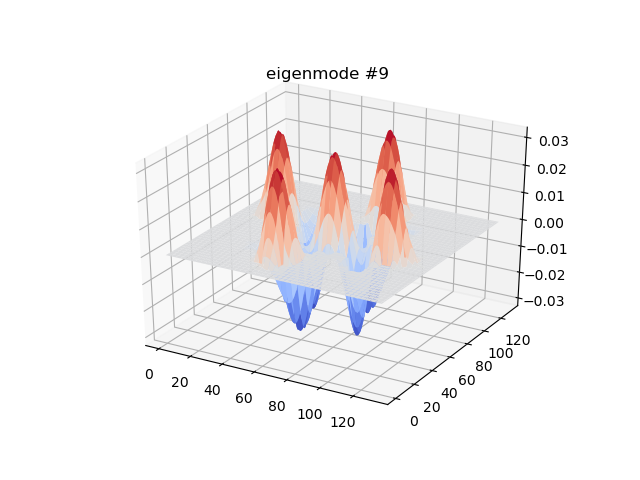
\includegraphics[width=\linewidth]{../figs/eigenmode_3d9.png}
    \end{subfigure}
    \begin{subfigure}{0.3\textwidth}
        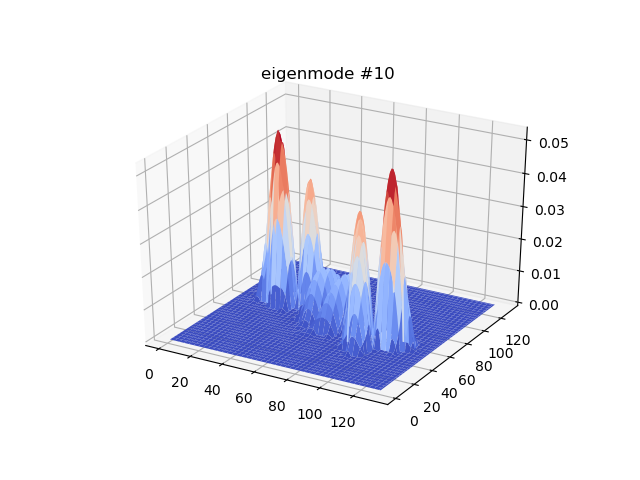
\includegraphics[width=\linewidth]{../figs/eigenmode_3d10.png}
    \end{subfigure}
    \caption{The 10 lowest eigenmodes, 3D plots.}
    \label{3dmodes}
\end{figure}

\end{document}

